\documentclass{beamer}

\usepackage{amssymb}
\usepackage{amsmath}
\usepackage{amsthm}
\usepackage{amsfonts}

\usepackage{multicol}

\usepackage{graphicx}
\graphicspath{ {./src} }

\usepackage{tikz}

\usepackage{pgfplots}
\pgfplotsset{compat = newest}

\usepackage{verbatim}
\usetikzlibrary{arrows,shapes}

% for cross reference
% \usepackage{hyperref}

% for fixed length of cell of tables
% \usepackage{tabularx}
% \usepackage{longtable}

\AtBeginSection[]
{
  \begin{frame}
    \frametitle{Table of Contents}
    \tableofcontents[currentsection]
  \end{frame}
}


\title{Communicate Without Errors}
\author{Zifan Hua}

\begin{document}

  % TODO use block theme for definitions and lemma

  \frame{\titlepage}

  \begin{frame}
        \frametitle[TOC]{Table Of Contents}
        \tableofcontents
  \end{frame}

  \section{Introduction}

\begin{frame}
      \frametitle{Introduction}
      \begin{itemize}
            \item Channel Capacity
            \item Zero Error Rate
            \item Shannon Capacity
            \item $C_{n}$
            \item $\sqrt{5} \le \Theta(C_{5}) \le 5/2$
            \item $\Theta(G) = \sqrt{5}$ by Lovász László
      \end{itemize}
\end{frame}

  \section{Basic Definitions}

% TODO rearrange the order of the definitions

\subsection{\texorpdfstring{Channel \& Graph}{Channel and Graph}}

\subsubsection*{Channel}

      \begin{frame}
            \frametitle{Channel}
            \begin{definition}[channel]
                  Characters is a finite set.

                  A message is a finite sequence of characters.

                  A channel has a sender and a receiver.
                  The sender sends a message to the receiver.
                  \begin{figure}[h!]
                        \tikzstyle{vertex}=[fill=black!25,minimum size=20pt,inner sep=0pt]
                        \tikzstyle{message}=[inner sep=0pt]
                        \tikzstyle{edge} = [draw,thick,-]
                        \tikzstyle{weight} = [font=\small]
                        \begin{tikzpicture}[scale=1, auto,swap]
                              % Draw a 7,11 network
                              % First we draw the vertices
                              \foreach \pos/\name in {{(0,0)/sender}, {(3,0)/receiver}}
                                    \node[vertex] (\name) at \pos {$\name$};
                              \foreach \pos/\name/\la in {{(0,0.7)/abcde/a\textbf{\textit{bc}}de}, {(3,0.7)/acbde/a\textbf{\textit{cb}}de}}
                                    \node[message] (\name) at \pos {\la};
                              % Connect vertices with edges and draw weights
                              \foreach \source/ \dest in {sender/receiver}
                              \path[edge] (\source) -- node[weight]{} (\dest);
                        \end{tikzpicture}
                  \end{figure}
                  \pause
                  
                  The receiver receives message and decode it.
                  \pause

                  However, in the procedure of send and receive, the channel may introduce some errors. For instance, here, character $b$ is decoded into $c$. 
            \end{definition}
      \end{frame}

\subsubsection*{Confusable}

      \begin{frame}
            \frametitle{Confusable}
            \begin{definition}[confusable]
                  Given two distinct characters $a$, $b$. If $a$ and $b$ have chance to be \textbf{decoded into a same character} say $c$, we say $a$ and $b$ are \textbf{confusable}.

                  For a two distinct messages of length $n$, say $a_{1}a_{2}\dots a_{n}$, $b_{1}b_{2}\dots b_{n}$ is confusable if and only if $a_{i}$ and $b_{i}$ are \textbf{confusable} or \textbf{same} for every $i$.
            \end{definition}
      \end{frame}

\subsubsection*{Rate of Channel}

      \begin{frame}
            \frametitle{Rate of Channel}

            \begin{definition}[rate of channel]
                  The rate of channel actually represent how many \textbf{distinct character} can be send \textbf{per unit time}.

                  Given a channel that could send $r$ distinct characters per unit time. And send message for $n$ unit time, so the number of distinct messages the channel can send is $r^{n}$.

                  \pause

                  \vspace{0.5em}

                  Conversely, given a channel that could send $m$ \textbf{distinct messages} in $n$ \textbf{unit time}.
                  Then the rate of channel is $\sqrt[n]{m}$.
                  
            \end{definition}
      \end{frame}

\subsubsection*{Zero Error Rate of Channel}

      \begin{frame}
            \frametitle{Zero Error Rate of Channel}
            \begin{definition}[zero error rate]
                  Given a channel that could send messages in $n$ unit time.

                  We want to find the maximum set of messages $M$ that \textbf{no two of them is confusable}.
                  Which means if we send these messages then, there is no chance of get an error.

                  \begin{equation}
                        \text{zero error rate} = \max_{M} \sqrt[n]{|M|}
                  \end{equation}
            \end{definition}
      \end{frame}

      \begin{frame}
            \frametitle{Zero Error Rate of Channel}
            
            \begin{definition}
                  If given a set of characters $S$, and some of the characters could be confusable.

                  In the reality, we usually do not fix $n$, so the thing we really want to find is
                  
                  \begin{equation}
                        \sup_{n} \left\{
                              \text{zero error rate of channel send messages for $n$ unit time}
                        \right\}
                  \end{equation}

                  And we call this the shannon Capacity and denoted by $\Theta(S)$.
            \end{definition}

            Clearly, shannon Capacity is actually a function of the set of characters. So, we want a more abstract way to represent the characters.
      \end{frame}

\subsubsection*{Graph}

\begin{frame}
      \frametitle{Graph Representation Of Characters}
      \begin{definition}[graph] \label{def:graph}
            A graph $ G $ is a set of vertices with a set of edges connecting pairs of vertices.

            \begin{figure}[h!]
                  \tikzstyle{vertex}=[circle,fill=black!25,minimum size=20pt,inner sep=0pt]
                  \tikzstyle{edge} = [draw,thick,-]
                  \tikzstyle{weight} = [font=\small]
                  \begin{tikzpicture}[scale=1, auto,swap]
                        % Draw a 7,11 network
                        % First we draw the vertices
                        \foreach \pos/\name in {{(0,2)/a}, {(2,1)/b}, {(4,1)/c},
                              {(0,0)/d}, {(3,0)/e}, {(2,-1)/f}, {(4,-1)/g}}
                              \node[vertex] (\name) at \pos {$\name$};
                        % Connect vertices with edges and draw weights
                        \foreach \source/ \dest in {b/a, c/b,d/a,d/b,
                              e/b, e/c,e/d,
                              f/d,f/e,
                              g/e,g/f}
                        \path[edge] (\source) -- node[weight]{} (\dest);
                  \end{tikzpicture}
                  \label{fig:graphDefinitionExample}
                  \caption{An example of a graph.}
            \end{figure}
      \end{definition}
\end{frame}

\begin{frame}
      \frametitle{Graph Representation Of Characters}
      \begin{definition}\label{def:graphRepresetationOfChannel}
            Given a channel that sending $\{1,2,\dots,n\}$ as characters. And some characters $i$ and $j$ could be confused with each other.

            \smallskip

            Then the graph representation of the characters is the graph with vertices $\{1,2,\dots,n\}$ and edges $(i,j)$ if and only if $i$ and $j$ is \textbf{distinct} and could be \textbf{confused with each other}.
      \end{definition}

      Accordingly, there is the corresponding way that using graphs to represent a message and Shannon Capacity.
\end{frame}

\begin{frame}
      \frametitle{Product Graph}
      
      The product of two graphs can be considered as send a pair of characters $(x,y)$ as one message. So, we have a channel that send messages of for $2$ unit time.

      \pause
      \smallskip

      Recall that before, $2$ distinct messages is confusable means that they can be decoded into the same message, which means every characters the two channel use need to be confusable or the same.

      \begin{definition}[graph product]\label{def:graphProduct}
            Given two graph $ G $ and $ H $. The graph product $ G \times H $ is the graph with vertices $ V(G \times H) = V(G) \times V(H) $ in which $ (x,y) $ is adjacent to $ (x',y') $ in $ G \times H $ if and only if $ x $ is \textbf{adjacent} to $ x' $ or the \textbf{same} in $ G $ and $ y $ is \textbf{adjacent} to $ y' $ or the \textbf{same} in $ H $.

            \pause

            A graph $ G $ product itself for $ n $ times will always be denoted by $ G^n $.

            Which means we could use $ G^n $ to represent messages of a channel that send messages for $n$ unit time.
      \end{definition}
\end{frame}

\begin{frame}
      \frametitle{$\alpha(G)$}
      \begin{definition}[$\alpha(G)$]\label{def:alpha}
            Given a finite graph $G$. $\alpha(G)$ is the \textbf{maximum} number of vertices such that every two of them is not adjacent in $G$.

            If $G$ represent a set of characters, $\sqrt[n]{\alpha(G^{n})}$ is just the zero error rate we have defined before.

            \pause

            \tikzstyle{vertex}=[circle,fill=black!25,minimum size=20pt,inner sep=0pt]
            \tikzstyle{selected vertex}=[circle,fill=red!25,minimum size=20pt,inner sep=0pt]
            \tikzstyle{edge} = [draw,thick,-]
            \tikzstyle{weight} = [font=\small]
            \begin{figure}[h!]
                  \begin{tikzpicture}[scale=1, auto,swap]
                        % Draw a 7,11 network
                        % First we draw the vertices
                        \foreach \pos/\name in {{(0,1)/a}, {(2,1)/b}, {(4,1)/c},
                              {(0,0)/d}, {(3,0)/e}, {(2,-1)/f}, {(4,-1)/g}}
                              \node[vertex] (\name) at \pos {$\name$};
                        \foreach \pos/\name in {{(0,1)/a}, {(4,1)/c},
                              {(2,-1)/f}}
                              \node[selected vertex] (\name) at \pos {$\name$};
                        % Connect vertices with edges and draw weights
                        \foreach \source/ \dest in {b/a, c/b,d/a,d/b,
                              e/b, e/c,e/d,
                              f/d,f/e,
                              g/e,g/f}
                        \path[edge] (\source) -- node[weight]{} (\dest);
                  \end{tikzpicture}
                  \label{fig:alphaGExample}
                  \caption{Example of $ \alpha(G) $. Here $ \alpha(G) = 3 $.}
            \end{figure}
      \end{definition}
\end{frame}


\subsection{Shannon Capacity}

\begin{frame}
      \frametitle{Shannon Capacity}
      \begin{definition}[Shannon Capacity]\label{def:shannonCapacity}
            Recall that Shannon Capacity is 
            \begin{equation}
                  \sup_{n} \left\{
                        \text{zero error rate of channel send messages for $n$ unit time}
                  \right\}
            \end{equation}

            Use the graph $G$ to represent the set of characters, the Shannon capacity $ \Theta(G) $ is defined by
            \begin{equation}
                  \Theta(G) = \sup_{n} \sqrt[n]{\alpha(G^n)} 
            \end{equation}

      \end{definition}
\end{frame}


  \section{The Main Solution}

      \begin{frame}
            To get the final result, we still need some more tools.
      \end{frame}

      \subsection{\texorpdfstring{Lower Bound of $\Theta(C_{5})$}{Lower Bound of Theta(C5)}}

\begin{frame}
      \frametitle{Lower Bound of $\Theta(C_{5})$}

      \begin{figure}[h!]
            \tikzstyle{vertex}=[circle,fill=black!25,minimum size=20pt,inner sep=0pt]
            \tikzstyle{edge} = [draw,thick,-]
            \tikzstyle{weight} = [font=\small]
            \begin{tikzpicture}[scale=1, auto,swap]
                  % Draw a 7,11 network
                  % First we draw the vertices
                  \foreach \pos/\name/\la in {{(0,2)/a/$v_{1}$},
                  {(1.902113032590307,0.6180339887498949)/b/$v_{2}$},
                  {(1.1755705045849465,-1.6180339887498947)/c/$v_{3}$},
                  {(-1.175570504584946,-1.618033988749895)/d/$v_{4}$},
                  {(-1.9021130325903073,0.6180339887498945)/e/$v_{5}$}}
                        \node[vertex] (\name) at \pos {\la};
                  % Connect vertices with edges and draw weights
                  \foreach \source/ \dest in {a/b,b/c,c/d,d/e,e/a}
                  \path[edge] (\source) -- node[weight]{} (\dest);
            \end{tikzpicture}
            \label{fig:Pentagon}
            \caption{$C_{5}$}
      \end{figure}

      The $ \alpha(C_{5}) $ is clearly equal to 2.

      \pause

      We want to show that $ \alpha((C_{5})^2) \ge 5 $.

      Thus $ \Theta(C_{5}) = \sup\sqrt[n]{(C_{5})^{n}} \ge \sqrt{\alpha((C_{5})^2)} \ge \sqrt{5} $
      
\end{frame}

\begin{frame}
      \frametitle{Lower Bound of $\Theta(C_{5})$}

      \begin{figure}[h!]
            \tikzstyle{vertexin}=[circle,fill=red!25,minimum size=20pt,inner sep=0pt]
            \tikzstyle{vertexout}=[circle,fill=green!25,minimum size=20pt,inner sep=0pt]
            \tikzstyle{edge} = [draw,thick,-]
            \tikzstyle{weight} = [font=\small]
            \begin{tikzpicture}[scale=1, auto,swap]
                  \foreach \i in {1,2,3,4,5}
                        \foreach \j in {1,2,3,4,5}
                              \node[vertexin] (v_{\i\j}) at (\i,\j) {$v_{\i\j}$};
                  
                  \node[vertexout] (v_{00}) at (0,0) {$v_{55}$};
                  \node[vertexout] (v_{01}) at (0,1) {$v_{51}$};
                  \node[vertexout] (v_{02}) at (0,2) {$v_{52}$};
                  \node[vertexout] (v_{03}) at (0,3) {$v_{53}$};
                  \node[vertexout] (v_{04}) at (0,4) {$v_{54}$};
                  \node[vertexout] (v_{05}) at (0,5) {$v_{55}$};

                  \node[vertexout] (v_{06}) at (0,6) {$v_{51}$};
                  \node[vertexout] (v_{16}) at (1,6) {$v_{11}$};
                  \node[vertexout] (v_{26}) at (2,6) {$v_{21}$};
                  \node[vertexout] (v_{36}) at (3,6) {$v_{31}$};
                  \node[vertexout] (v_{46}) at (4,6) {$v_{41}$};
                  \node[vertexout] (v_{56}) at (5,6) {$v_{51}$};

                  \node[vertexout] (v_{66}) at (6,6) {$v_{11}$};
                  \node[vertexout] (v_{65}) at (6,5) {$v_{15}$};
                  \node[vertexout] (v_{64}) at (6,4) {$v_{14}$};
                  \node[vertexout] (v_{63}) at (6,3) {$v_{13}$};
                  \node[vertexout] (v_{62}) at (6,2) {$v_{12}$};
                  \node[vertexout] (v_{61}) at (6,1) {$v_{11}$};

                  \node[vertexout] (v_{60}) at (6,0) {$v_{15}$};
                  \node[vertexout] (v_{50}) at (5,0) {$v_{55}$};
                  \node[vertexout] (v_{40}) at (4,0) {$v_{45}$};
                  \node[vertexout] (v_{30}) at (3,0) {$v_{35}$};
                  \node[vertexout] (v_{20}) at (2,0) {$v_{25}$};
                  \node[vertexout] (v_{10}) at (1,0) {$v_{15}$};
            \end{tikzpicture}
            \label{fig:Pentagon2}
            \caption{$(C_{5})^{2}$}
      \end{figure}

\end{frame} 

\begin{frame}
      \frametitle{Lower Bound of $\Theta(C_{5})$}

      It is messy to draw edges in the graph of $(C_{5})^{2}$. So we use the following graph to give some idea of $(C_{5})^{2}$. But it is clear that every point is adjacent to the 8 points around it.

      Point $v_{ij}$ represent the vertex $(v_{i},v_{j})$ in $(C_{5})^{2}$.

      The green points are the same with the corresponding red points, we use it just for the convenience of visualization.

      \pause

      We will choose five points $v_{11}$, $v_{23}$, $v_{35}$, $v_{42}$, $v_{54}$, and show that they are mutually not adjacent.

\end{frame}

\begin{frame}
      \frametitle{Lower Bound of $\Theta(C_{5})$}

      \begin{figure}[h!]
            \tikzstyle{vertexin}=[circle,fill=red!25,minimum size=20pt,inner sep=0pt]
            \tikzstyle{vertexout}=[circle,fill=green!25,minimum size=20pt,inner sep=0pt]
            \tikzstyle{vertexs}=[circle,fill=blue!25,minimum size=20pt,inner sep=0pt]
            \tikzstyle{edge} = [draw,thick,-]
            \tikzstyle{weight} = [font=\small]
            \begin{tikzpicture}[scale=1, auto,swap]
                  \foreach \i in {1,2,3,4,5}
                        \foreach \j in {1,2,3,4,5}
                              \node[vertexin] (v_{\i\j}) at (\i,\j) {$v_{\i\j}$};
                  
                  \node[vertexout] (v_{00}) at (0,0) {$v_{55}$};
                  \node[vertexout] (v_{01}) at (0,1) {$v_{51}$};
                  \node[vertexout] (v_{02}) at (0,2) {$v_{52}$};
                  \node[vertexout] (v_{03}) at (0,3) {$v_{53}$};
                  \node[vertexout] (v_{04}) at (0,4) {$v_{54}$};
                  \node[vertexout] (v_{05}) at (0,5) {$v_{55}$};

                  \node[vertexout] (v_{06}) at (0,6) {$v_{51}$};
                  \node[vertexout] (v_{16}) at (1,6) {$v_{11}$};
                  \node[vertexout] (v_{26}) at (2,6) {$v_{21}$};
                  \node[vertexout] (v_{36}) at (3,6) {$v_{31}$};
                  \node[vertexout] (v_{46}) at (4,6) {$v_{41}$};
                  \node[vertexout] (v_{56}) at (5,6) {$v_{51}$};

                  \node[vertexout] (v_{66}) at (6,6) {$v_{11}$};
                  \node[vertexout] (v_{65}) at (6,5) {$v_{15}$};
                  \node[vertexout] (v_{64}) at (6,4) {$v_{14}$};
                  \node[vertexout] (v_{63}) at (6,3) {$v_{13}$};
                  \node[vertexout] (v_{62}) at (6,2) {$v_{12}$};
                  \node[vertexout] (v_{61}) at (6,1) {$v_{11}$};

                  \node[vertexout] (v_{60}) at (6,0) {$v_{15}$};
                  \node[vertexout] (v_{50}) at (5,0) {$v_{55}$};
                  \node[vertexout] (v_{40}) at (4,0) {$v_{45}$};
                  \node[vertexout] (v_{30}) at (3,0) {$v_{35}$};
                  \node[vertexout] (v_{20}) at (2,0) {$v_{25}$};
                  \node[vertexout] (v_{10}) at (1,0) {$v_{15}$};

                  \node[vertexs] (v_{11}) at (1,1) {$v_{11}$};
                  \node[vertexs] (v_{66}) at (6,6) {$v_{11}$};
                  \node[vertexs] (v_{16}) at (1,6) {$v_{11}$};
                  \node[vertexs] (v_{61}) at (6,1) {$v_{11}$};

                  \node[vertexs] (v_{23}) at (2,3) {$v_{23}$};

                  \node[vertexs] (v_{35}) at (3,5) {$v_{35}$};
                  \node[vertexs] (v_{30}) at (3,0) {$v_{35}$};

                  \node[vertexs] (v_{42}) at (4,2) {$v_{42}$};

                  \node[vertexs] (v_{54}) at (5,4) {$v_{54}$};
                  \node[vertexs] (v_{04}) at (0,4) {$v_{54}$};

            \end{tikzpicture}
            \label{fig:Pentagon3}
            \caption{$(C_{5})^{2}$}
      \end{figure}

\end{frame}

      \subsection{Alpha Function of Product Graph}

\begin{frame}
      \frametitle{Alpha Function of Product Graph}
      \begin{lemma}
            $\alpha(G)\alpha(H) \leq \alpha(G \times H)$
      \end{lemma}

      \pause

      \begin{proof}
            Given graph $ G $ and $ H $. Let $ G' $ and $ H' $ be subgraph of $ G $ and $ H $ such that no vertex of $ G' $ or $ H' $ is adjacent in $ G $ or $ H $, respectively. Then $ G' \times H' $ is a subgraph of $ G \times H $ such that no vertex of $ G' \times H' $ is adjacent in $ G \times H $.
      \end{proof}
\end{frame}

      \subsection{Orthonormal Representation}

      \begin{frame}
            \frametitle{Orthonormal Representation}

            Here we have the third way to defined a set of characters.

            \begin{definition}[Orthonormal Representation]\label{def:orthonormalRepresentation}
                  Given a graph $ G $ with vertices $ 1,2,\dots,n $, the orthonormal representation of $ G $ is a set of unit vectors $ \{v_1, v_2, \dots, v_n\} $ such that $ v_i $ and $ v_j $ are orthogonal if $ i $ and $ j $ are not adjacent in $ G $.
            \end{definition}

            \pause

            This existence of the orthonormal representation can be proved by induction.

      \end{frame}

\subsection{Tensor Product}

      \begin{frame}
            \frametitle{Tensor Product}
            \begin{definition}[tensor product]\label{def:tensorProduct}
                  Given two vectors $ v = \left(v_{1},\dots,v_{n}\right) $ and $ w = \left(w_{1},\dots,w_{n}\right) $, the tensor product $ v \circ w $ is defined by
                  \begin{equation}
                        v \circ w = \left(
                              v_{1}w_{1},\dots,v_{1}w_{n},
                              v_{2}w_{1},\dots,v_{2}w_{n},
                              \dots,
                              v_{n}w_{1},\dots,v_{n}w_{n}
                              \right)
                  \end{equation}
            \end{definition}

            \pause

            \begin{lemma}
                  The inner product of tensor products can be computed by,
                  \begin{equation}
                        \langle v \circ w, v' \circ w' \rangle = \langle v, v' \rangle \langle w, w' \rangle
                  \end{equation}
            \end{lemma}

      \end{frame}

      \begin{frame}
            This is the product of graph in the sense of orthonormal representation.

            \frametitle{Product of Orthonormal Representation}
            \begin{lemma}
                  Given a graph $ G $ with vertices $ 1,2,\dots,n $, and a graph $ H $ with vertices $ 1,2,\dots,m $. Then vectors $\{ v_{i}\circ w_{j} \}$ is an orthonormal representation of $ G \times H $.
            \end{lemma}
      \end{frame}

      \subsection{Theta Function}

      \begin{frame}
            \frametitle{Theta Function}
            Given a graph $ G $, the $ \theta(G) $ is defined by
            \begin{equation}
                  \theta(G) = \inf_{\{v_1, v_2, \dots, v_n\},c} \max_{i} \frac{1}{\left<c,v_{i}\right>^2}
            \end{equation}
            where $ \{v_1, v_2, \dots, v_n\} $ is an orthonormal representation of $ G $, and c is any unit vector does not orthogonal to $ v_i $.

            \pause

            \begin{lemma}
                  There always exist such an $c$ and orthonormal representation $ \{v_1, v_2, \dots, v_n\} $ such that
                  \begin{equation}
                        \theta(G) = \max_{i} \frac{1}{\left<c,v_{i}\right>^2}
                  \end{equation}
            \end{lemma}

            This could be proved by proving the set of all possible cases of $ \{v_1, v_2, \dots, v_n,c \} $ is compact. And the function $ \max \frac{1}{\left<c,v_{i}\right>^2} $ is continuous.
      \end{frame}

\subsection{Theta Function of Product Graph}

      \begin{frame}
            \frametitle{Theta Function of Product Graph}
            \begin{lemma}
                  Given graph $ G $ and $ H $, then
                  \begin{equation}
                        \theta(G \times H) \leq \theta(G) \theta(H)
                  \end{equation}
            \end{lemma}

            \pause

            \begin{proof}
                  Let $ \{v_1, v_2, \dots, v_n\} $ and $ \{w_1, w_2, \dots, w_m\} $ be orthonormal representation of $ G $ and $ H $ and $ c_{v} $ and $ c_{w} $ such that
                  \begin{equation}
                        \max \left\{ \frac{1}{\left<c_{v},v_{i}\right>^2} : i=1,2,\dots,n \right\} = \theta(G)
                  \end{equation} 
                  and 
                  \begin{equation}
                        \max \left\{ \frac{1}{\left<c_{w},w_{i}\right>^2} : i=1,2,\dots,m \right\} = \theta(H)
                  \end{equation}
            \end{proof}
      \end{frame}

      \begin{frame}
            \begin{proof}
                  Then
                  \begin{eqnarray}
                        \theta(G \times H) &\leq& 
                        \max \left\{ \frac{1}{\left<c_{v} \circ c_{w},v_{i} \circ w_{j}\right>^2} \right\} \\
                        &=& \max \left\{ \frac{1}{\left<c_{v},v_{i}\right>^2 \left<c_{w},w_{j}\right>^2} \right\} \\
                        &=& \max \left\{ \frac{1}{\left<c_{v},v_{i}\right>^2} \right\} \max \left\{ \frac{1}{\left<c_{w},w_{j}\right>^2} \right\} \\
                        &=& \theta(G) \theta(H) \\
                  \end{eqnarray}
            \end{proof}
      \end{frame}

\subsection*{Relation of Theta Function and Alpha Function}

      \begin{frame}
            \frametitle{Relation of Theta Function and Alpha Function}

            \begin{lemma}
                  \begin{equation}
                        \theta(G) \geq \alpha(G)
                  \end{equation}
            \end{lemma}

            \pause

            \begin{proof}
                  Let $ \{1,2,\dots,k\} $ be the set of vertices of $ G $ such that every point is not adjacency in $ G $. And $ k = \alpha(G) $
      
                  Let $ \{v_1, v_2, \dots, v_n\} $ be an orthonormal representation of $ G $ and $ c $ such that
                  \begin{equation}
                        \max \left\{ \frac{1}{\left<c,v_{i}\right>^2} \right\} = \theta(G)
                  \end{equation}
                        
                  Then
                  \begin{eqnarray}
                        1 &=& c^{2}
                        \geq \sum_{i=1}^{k} \left<c,v_{i}\right>^{2}
                        \geq \frac{k}{\theta(G)}
                  \end{eqnarray}
            \end{proof}
      \end{frame}

\subsection*{Relation of Theta Function and Shannon Capacity}
      
      \begin{frame}
            \frametitle{Relation of Theta Function and Shannon Capacity}

            \begin{theorem}
                  Given a graph $ G $, then
                  \begin{equation}
                        \theta(G) \geq \Theta(G)
                  \end{equation}
            \end{theorem}

            \pause

            \begin{proof}
                  % TODO fix the issue of the proof by change lim to sup
                  \begin{eqnarray}
                        \Theta(G) &=& \lim_{n} \sqrt[n]{\alpha(G^{n})} \\
                        &\leq& \lim_{n} \sqrt[n]{\theta(G^{n})} \\
                        &\leq& \lim_{n} \sqrt[n]{\theta(G)^{n}} \\
                        &=& \theta(G)
                  \end{eqnarray}
            \end{proof}
      \end{frame}

      \begin{frame}
            The final result we want to prove today,
            \begin{equation}
                  \Theta(C_{5}) \le \theta(C_{5}) \le \sqrt{5}
            \end{equation}
      \end{frame}

      \subsection{Final Result}

\begin{frame}
      \begin{theorem}
            \begin{equation}
                  \theta(C_{n}) \leq \sqrt{5}
            \end{equation}
      \end{theorem}
\end{frame}

\begin{frame}
      \begin{proof}
            Consider an umbrella that has a handle and $5$ ribs that all have unit length. And also its handle is a unit vector.

            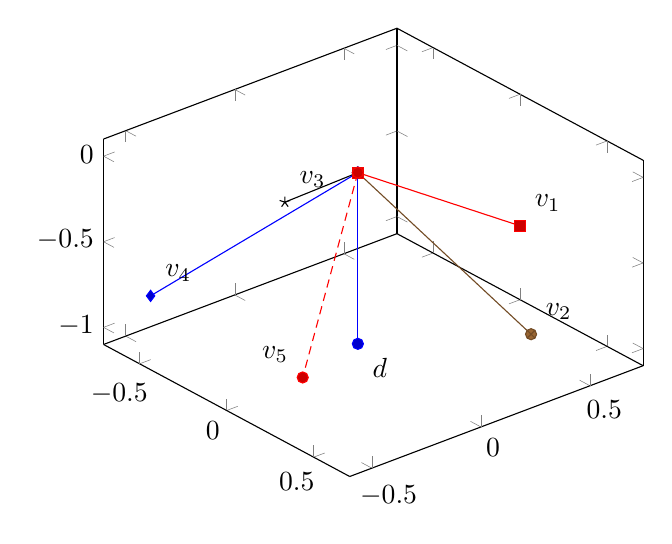
\begin{tikzpicture}
                  \begin{axis}[view = {50}{40}]
                        
                  \addplot3 coordinates 
                  {
                        (0,0,0)
                        (0,0,-1)
                  };

                  \node[below right, outer sep=2pt] at (0,0,-1) {$d$};

                  \addplot3 coordinates 
                  {
                        (0,0,0)
                        (0,0.74349606,-0.66874031)
                  };

                  \node[above right, outer sep=2pt] at (0,0.74349606,-0.66874031) {$v_{1}$};
                        
                  \addplot3 coordinates 
                  {
                        (0,0,0)
                        (0.70710677,0.22975292,-0.66874031)
                  };

                  \node[above right, outer sep=2pt] at (0.70710677,0.22975292,-0.66874031) {$v_{2}$};

                  \addplot3 coordinates 
                  {
                        (0,0,0)
                        (-0.70710677,0.22975292,-0.66874031)
                  };

                  \node[above right, outer sep=2pt] at (-0.70710677,0.22975292,-0.66874031) {$v_{3}$};

                  \addplot3 coordinates 
                  {
                        (0,0,0)
                        (-0.43701602,-0.60150095,-0.66874031)
                  };

                  \node[above right, outer sep=2pt] at (-0.43701602,-0.60150095,-0.66874031) {$v_{4}$};
                  
                  \addplot3 coordinates 
                  {
                        (0,0,0)
                        (0.43701602,-0.60150095,-0.66874031)
                  };

                  \node[above left, outer sep=2pt] at (0.43701602,-0.60150095,-0.66874031) {$v_{5}$};

                  \end{axis}
                        
            \end{tikzpicture}

      \end{proof}
\end{frame}

\begin{frame}
      \begin{proof}
            Here, angles between two consecutive ribs are same. 
            
            Let $v$ be a rib. And let $w$ be one of the rib that have the largest angle with $v$. Then, we let the angle between $v$ and $w$ be $ \pi/2 $.

            Then, the $5$ ribs of such an umbrella form an orthonormal representation of $C_{5}$.

            Let $d$ be the vector represent the handle, and $v_{1},v_{2},\dots,v_{5}$ be the $5$ ribs. And let $\gamma$ be the angle between the handle and any rib.

            So, by some calculation, we get
            \begin{eqnarray}
                  \theta(C_{5}) &\le& \max \frac{1}{<d,v_{i}>^{2}} \\
                  &=& \left(
                        \frac{1}{\cos(\gamma)}
                  \right)^{2} \\
                  &=& \sqrt{5}
            \end{eqnarray}
      \end{proof}
\end{frame}

  
  \section{Conclusion and Discussion}

\begin{frame}
      \frametitle{Conclusion}
      \begin{itemize}
            \item We have proved that $Theta(C_{5}) = \sqrt{5}$
            \item We could actually proved that $\Theta(C_{n})$ is equal to $ n\frac{\cos(\pi/n)}{1+\cos(\pi/n)} $.
      \end{itemize}
\end{frame}

\begin{frame}
      \frametitle{Open Questions}
      \begin{itemize}
            \item Although $\Theta(C_{n})$ is equal to $ n\frac{\cos(\pi/n)}{1+\cos(\pi/n)} $, but we still don't know the exact value of $\Theta(C_{n})$. Even for $n=7$
            \item Is there any good lower bound for $\Theta(C_{n})$?
            \item Is there any patterns for $n$ such that $\Theta(c_{n})$ is hard to compute?
      \end{itemize}
\end{frame}

\begin{frame}
      \frametitle{Discussion}

      In the real world cases, we always have some kind of relay between the sender and receiver. So the new channel is kind of composite of two channel. Can we compute Shannon Capacity these channels independently and then combine them together to get the Shannon Capacity of the new Channel?
\end{frame}

\section{Reference}

\begin{frame}
      \frametitle{Reference}
      \begin{itemize}
            \item \href{https://ieeexplore.ieee.org/stamp/stamp.jsp?arnumber=1055985}{On the Shannon Capacity of a Graph} by Laszlo Lovasz
            \item \href{https://ieeexplore.ieee.org/stamp/stamp.jsp?tp=&arnumber=1056798}{The zero error capacity of a noisy channel} by Claude Shannon
      \end{itemize}
\end{frame}

\end{document}